\documentclass[journal]{IEEEtran}

% *** CITATION PACKAGES ***
\usepackage{cite}
\usepackage{float}
\usepackage{tabularx}
% *** MATH PACKAGES ***
\usepackage{amsmath,amssymb,amsfonts}

% *** GRAPHICS RELATED PACKAGES ***
\ifCLASSINFOpdf
  \usepackage[pdftex]{graphicx}
  \graphicspath{{figures/}}
  \DeclareGraphicsExtensions{.pdf,.jpeg,.png}
\else
  \usepackage[dvips]{graphicx}
  \graphicspath{{figures/}}
  \DeclareGraphicsExtensions{.eps}
\fi

% *** SPECIALIZED LIST PACKAGES ***
\usepackage{algorithm}
\usepackage{algpseudocode}

% *** ALIGNMENT PACKAGES ***
\usepackage{array}

% *** FLOAT PACKAGES ***
\usepackage{stfloats}

% *** PDF, URL AND HYPERLINK PACKAGES ***
\usepackage[colorlinks=true, linkcolor=black, citecolor=black, urlcolor=blue]{hyperref}

% *** ADDITIONAL PACKAGES ***
\usepackage{textcomp}
\usepackage{xcolor}
\usepackage{booktabs}
\usepackage{multirow}
\usepackage{tabularx}
\usepackage{tikz}
\usetikzlibrary{arrows.meta, positioning, shapes.geometric, fit, backgrounds}
\usepackage{placeins}

\usepackage{etoolbox}
\makeatletter
\patchcmd{\@makecaption}{\scshape}{}{}{}
\makeatother

\def\BibTeX{{\rm B\kern-.05em{\sc i\kern-.025em b}\kern-.08em
    T\kern-.1667em\lower.7ex\hbox{E}\kern-.125emX}}

\hyphenation{op-tical net-works semi-conduc-tor}

\begin{document}

\title{Federated Learning for ICU Mortality Prediction on Heterogeneous Clinical Data}

\author{
    \IEEEauthorblockN{
      Md. Raiyan Ur Rahman Jiyon\textsuperscript{1},
        Md. Naimul Islam\textsuperscript{1}, Mohammad Shorif Uddin\textsuperscript{1,2}, \\
    }

    \IEEEauthorblockA{\textsuperscript{1}Department of Computer Science and Engineering, Green University of Bangladesh, Dhaka, Bangladesh\\
    \textsuperscript{2}Department of Computer Science and Engineering, Jahangirnagar University, Savar, Dhaka, Bangladesh}
    
    
    \IEEEauthorblockN{Emails: 
    raiyanjiyon@gmail.com, nayemhasan1314@gmail.com, shorifuddin@juniv.edu}   
}

% The paper headers
\markboth{IEEE Journal of Biomedical and Health Informatics,~Vol.~XX, No.~XX, June~2026}%
{Jiyon et al.: Privacy-Preserving and Byzantine-Robust Federated Learning}

\maketitle

\begin{abstract}
 Privacy laws such as HIPAA (Health Insurance Portability and Accountability Act) and GDPR (General Data Protection Regulation) prevent hospitals from consolidating data, while isolated datasets fail to build effective predictive models. This research uses Federated Learning (FL) to develop a clinically usable ICU (Intensive Care Unit) mortality prediction model without revealing sensitive information, evaluating whether Byzantine-robust aggregation maintains model quality when hospitals are compromised.
 The MIMIC-IV (Medical Information Mart for Intensive Care IV) dataset containing 65,273 hospitalizations and 31 clinical parameters is partitioned into seven care units to simulate a heterogeneous multi-client Non-IID environment. We compare FedAvg, FedProx, Median, Krum, and F2-score weighted aggregation (FedF2). Differential privacy is enforced via DP-SGD (Differentially Private Stochastic Gradient Descent) with $\epsilon=4.36$ and $\delta=10^{-5}$.
 Centralized baseline achieves an AUROC (Area Under the Receiver Operating Characteristic Curve) of 0.8920 (85.2\% recall), while federated XGBoost yields 0.9155 AUROC and Platt-scaled federated logistic regression produces 0.8784. Under a 3-of-7 adversarial client attack, Median and Krum maintain AUROC $>$ 0.8594, whereas FedAvg drops to 0.5011. DP-SGD achieves 0.8477 AUROC after scaling, and external validation on the eICU-CRD (eICU Collaborative Research Database) dataset yields 0.8337 AUROC.
 Privacy-preserving federated learning with Byzantine-robust aggregations is clinically feasible for multi-hospital networks. Byzantine-robust algorithms such as Median and Krum must be used when client reliability cannot be assured, while FedAvg suffices when clients are fully trusted.
\end{abstract}

\begin{IEEEkeywords}
Federated Learning, Healthcare Machine Learning, Differential Privacy, Non-IID Data, Byzantine Robustness
\end{IEEEkeywords}

\begin{figure*}[t]
\centering
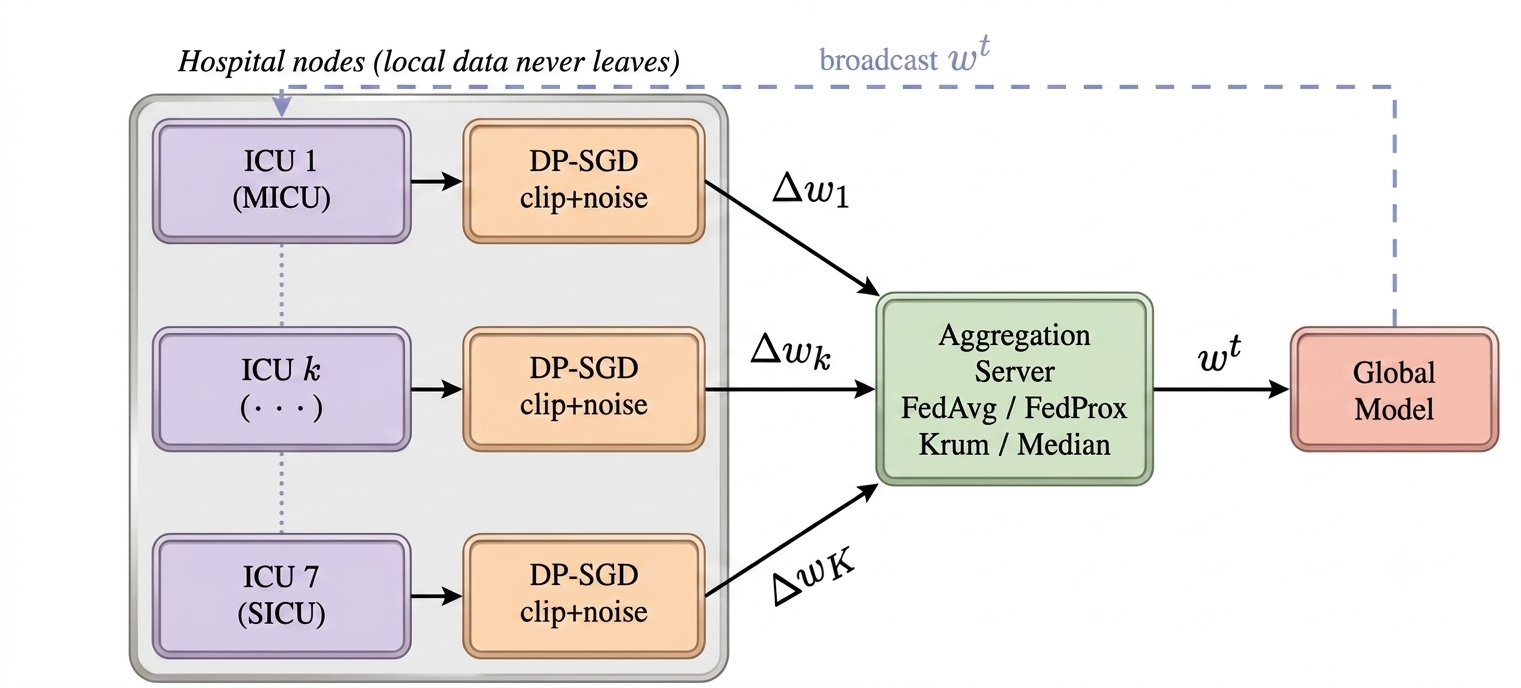
\includegraphics[width=0.95\textwidth]{fig.png}
\caption{Federated clinical learning architecture: 7 ICU care units train local mortality prediction models with DP-SGD (per-sample gradient clipping + calibrated Gaussian noise). Privatized model updates $\Delta w_k$ are sent to a central aggregation server, which applies Byzantine-robust aggregation (FedAvg, FedProx, Krum, or Median) and broadcasts the global model $w^t$ back to clients. No raw patient data or EHR records are transmitted. An aggregation server can tolerate compromised clients (e.g., due to ransomware or misconfiguration) by using robust aggregation methods.}
\label{fig:architecture}
\end{figure*}

\section{Introduction}
The healthcare industry has developed numerous mechanisms for collecting medical data in clinical institutions at an unprecedented rate, including electronic health records, radiology image storage, and laboratory test data. However, virtually no exchange of this data takes place between different healthcare organizations, primarily because existing legislation such as the Health Insurance Portability and Accountability Act (HIPAA) in the US and the General Data Protection Regulation (GDPR) in the European Union prohibits sharing patient data outside institutional boundaries~\cite{price2019privacy,wiens2019do}. Additionally, there has been a significant rise in ransomware attacks on hospital IT systems, increasing risks in centralized data storage~\cite{mothukuri2021survey}. Machine learning algorithms that require extensive datasets to train effectively cannot access them \cite{nguyen2022federated}.

Federated Learning (FL) was proposed precisely to work around this constraint \cite{mcmahan2017communication}. The idea is straightforward: data never moves. Instead, every participating hospital trains a local copy of the model and transmits only the resulting weight updates to a central server, which fuses them into a shared global model \cite{kairouz2021advances}.

Moving from controlled experiments to actual hospital networks, however, uncovers a stubborn problem. Most FL algorithms---Federated Averaging (FedAvg) chief among them---were designed with well-calibrated, Independent and Identically Distributed (IID) benchmarks in mind \cite{li2020federated_challenges}. Real clinical populations look nothing like that. A diabetes clinic in a metropolitan area and a rural general practice serve wildly different patient demographics; their local datasets are, statistically speaking, deeply Non-Independent and Identically Distributed (Non-IID) \cite{zhao2018federated}. When a server naively averages weights from such mismatched clients, the optimization process can destabilize: different hospitals effectively tug the model in opposite directions \cite{fedprox, scaffold}.

Additionally, there is a security dimension that requires consideration. FL avoids transmission of raw data, but the gradient updates that are indeed transmitted over the network contain sensitive information. Zhu et al. showed that under optimal settings, an attacker may reverse-engineer gradients to recover original training data records \cite{zhu2019deep}. Unless strict mathematical constraints are enforced on the model for privacy protection, this weakness remains open \cite{dwork2014algorithmic, abadi2016deep}. Prompted by such concerns, we have developed a privacy-aware FL pipeline using MIMIC-IV (Medical Information Mart for Intensive Care IV), a large ICU database. Using MIMIC-IV, we create heterogeneous client groups by partitioning the data into ICU (Intensive Care Unit) care units and evaluate our model for external validation on the eICU-CRD (eICU Collaborative Research Database) dataset from 7 independent hospitals. Our contributions include the following:
\begin{itemize}

\item We partition the MIMIC-IV dataset into seven ICU care units to construct realistic Non-IID clients, validating external generalizability on the multi-hospital eICU-CRD dataset.

\item We analyze Byzantine-robust aggregation methods (Median and Krum) under multiple poisoning attacks, demonstrating their robustness (AUROC $\geq$ 0.8594) compared to FedAvg and FedProx.

\item We evaluate the privacy-utility trade-offs of DP-SGD alongside multiple architectures and FedF2, showing that FedF2 is highly effective in trusted settings but vulnerable to Byzantine attacks.

\end{itemize}

\section{Related Work}

Federated Learning (FL) has emerged as a promising paradigm for collaborative healthcare analytics by enabling multiple institutions to train shared machine learning models without exchanging sensitive patient records. The effectiveness of FL has been demonstrated in numerous clinical applications, including brain tumor segmentation~\cite{sheller2020brain}, pneumonia detection with explainable AI~\cite{biswas2025flpnexainet}, COVID-19 outcome prediction across twenty hospitals~\cite{dayan2021federated}, rare cancer segmentation involving seventy-one institutions~\cite{pati2022federated}, as well as stroke prediction, drug discovery, and electronic health record (EHR) analysis~\cite{kaissis2020secure,xu2021federated}. Recently, Zhao et al.~\cite{zhao2025privacy} developed a privacy-preserving federated framework for multi-source EHR prognosis prediction using feature calibration. Although these studies demonstrate the feasibility of collaborative learning, they primarily evaluate FL under benign environments and often provide limited analysis of statistical heterogeneity, adversarial robustness, formal privacy guarantees, and external clinical validation. Xu et al.~\cite{xu2021federated}, for instance, reported that federated EHR models experience noticeable performance degradation when participating hospitals differ substantially in patient demographics, indicating that practical deployment remains challenging.

One of the most significant challenges in healthcare FL is the presence of Non-IID data. Li et al.~\cite{li2020convergence} theoretically showed that FedAvg suffers from unstable convergence under heterogeneous client distributions, while Zhao et al.~\cite{zhao2018federated} observed performance degradation of up to 55\% compared with centralized IID training. To address this issue, several optimization strategies have been proposed, including FedProx~\cite{fedprox}, SCAFFOLD~\cite{scaffold}, and personalized federated learning methods such as Ditto and MAML~\cite{li2021ditto,fallah2020personalized}. Clinical datasets introduce additional challenges, including severe class imbalance, missing values, and varying disease prevalence across hospitals, leaving the effectiveness of these optimization strategies in practical ICU settings insufficiently explored. To better reflect real-world hospital collaboration, our framework adopts FedProx and constructs realistic ICU-specific Non-IID client partitions using MIMIC-IV, followed by external validation on the eICU-CRD dataset.

Security and privacy remain equally important challenges because model updates themselves may leak sensitive patient information. Zhu et al.~\cite{zhu2019deep} demonstrated that original training samples can be reconstructed from shared gradients, while membership inference and model inversion attacks further expose patient information without direct access to the underlying datasets~\cite{shokri2016membership}. Differential Privacy (DP), particularly DP-SGD~\cite{abadi2016deep,dwork2014algorithmic}, has therefore become a standard mechanism for providing formal privacy guarantees, although stronger privacy often reduces predictive performance. In parallel, Byzantine-resilient aggregation methods such as Krum~\cite{blanchard2017machine} and coordinate-wise Median~\cite{yin2018byzantine} have been proposed to defend against malicious client updates with relatively low computational overhead. However, previous studies generally investigate privacy preservation, Byzantine robustness, and optimization independently, while most evaluations rely on synthetic benchmark datasets rather than realistic healthcare environments. Consequently, the combined impact of heterogeneous data, differential privacy, and Byzantine attacks on clinical prediction remains insufficiently understood. Our work addresses this gap by jointly evaluating DP-SGD, Krum, and coordinate-wise Median under realistic poisoning attacks and heterogeneous ICU federated learning settings.

\section{Methodology}

Our experiments were conducted by subjecting FL to conditions resembling real hospital network environments rather than standard benchmark settings (Fig. 1). There are four key parameters in our design of experiments: the way the distributed simulation was structured, the division of data for generating demographic diversity, the server-side aggregation countermeasures to employ, and the addition of privacy guarantees.

\subsection{System Architecture and Reproducibility}

All experiments use random seed 42 with stratified train–validation–test splits. We replicate chosen measurements five times using five random seeds (FedAvg: 0.8845 $\pm$ 0.0068).

\subsection{Distributed Patient Cohorts (Care-Unit Modeling)}

MIMIC-IV \cite{PhysioNet-mimiciv-3.1,johnson2023mimic} (version 3.1 of Medical Information Mart for
Intensive Care) ICU-specific database will be used in our work. It contains 65,273
patient ICU admissions data that are characterized by 31 variables. These variables include demographics (age, gender, type of admission, insurance type), vital signs recorded in the first 24-hour period (HR, SBP, MAP, RR, temperature, SpO$_2$, glucose), laboratory measurements (creatinine, BUN, sodium, potassium, bicarbonate, hemoglobin, WBC, platelet, lactate, bilirubin, INR), and
predictions of scores (SOFA, SAPS II \cite{knaus1985apache}, Charlson index \cite{charlson1987new}).

Federated learning on the MIMIC-IV dataset is well-suited to its heterogeneous nature. MIMIC-IV allows patient admissions to be split into 7 different ICU care units (MICU, SICU, CCU, etc.), where each unit serves a distinct patient population, resulting in Non-IID distributional heterogeneity. We used these 7 ICUs as our 7 federated clients to model a multi-client federated setting with Non-IID local data distributions.

\textbf{Scope of simulation.} We note that our experiment involves
7 clients originating from a common institution (Beth Israel
Deaconess Medical Center). While this approach allows for
controlled studies regarding the effect of Non-IID and robustness
to adversaries within the known partition setting, it does not mimic
fully the effect of heterogeneous hospitals due to differences in
EHR software systems, protocols, or patient demographics. Our
validation experiments in Section~\ref{subsec:eicu_validation} with eICU-CRD involve
geographically separate hospitals, which is the real-world test
setting.

\subsection{Model Architectures}

To confirm the ability of federated learning to generalize to more
complicated model architectures than simple linear regressions, we test the following architectures:

\paragraph{Logistic Regression (Baseline):}
Training is done for balanced logistic regression (31 features $\rightarrow$ 1 output) with $\ell_2$ regularization and class weights balancing because of the imbalance
between classes (11\%). The model is explainable, computationally cheap, and constitutes a classical statistical framework for medical machine learning problems.

\paragraph{Multi-Layer Perceptron (MLP).}
To examine whether federated learning preserves its ability to handle complex model architectures, we trained the MLP network (architecture $31 \rightarrow 64
\rightarrow 32 \rightarrow 1$, where input features are followed by two hidden layers with 64 and 32 neurons respectively and a binary output.
We apply ReLU activation on all neurons but the output, which
uses sigmoid activation. The training utilizes the Adam optimizer (learning rate equals 0.001) and binary cross-entropy loss
function. The number of iterations per one federated learning
round equals 20 epochs. Batch size is equal to 32 and remains
the same as in the case of logistic regression.
Training procedure uses the same splits and StandardScaler preprocessing method as logistic regression.

Both models have been trained using the same train/
validation/test splits, and threshold-calibrated recall optimization is used on the validation sets for each model.

\subsection{Federated Aggregation Approaches}

Perhaps the most straightforward approach to aggregating
updates from client devices by the server is simply averaging,
known as Federated Averaging or FedAvg \cite{mcmahan2017communication}. This method is prone to two kinds of problems related
to this paper. First, averaging in case of non-uniform data distribution among clients allows the majority
of clients to take control over the global model. Second, just
one malicious client is enough to spoil the whole aggregate.
For this reason, we explored the proximal approach FedProx in combination with robust aggregation schemes.

\subsection{Mathematical Formalism}

\subsubsection{Federated Learning with Byzantine Robustness and Privacy}

We formulate the federated learning problem as an Empirical Risk Minimization problem in the distributed setting. Assume that there are $K$ clients, where each client $k$ has its own data $\mathcal{D}_k$ of size $n_k$. The goal of the optimization problem is to minimize the loss:
\begin{equation}
\min_{\mathbf{w}} F(\mathbf{w}) = \frac{1}{n} \sum_{k=1}^{K} n_k \cdot F_k(\mathbf{w}), \quad n = \sum_{k=1}^{K} n_k.
\end{equation}

2) Performance-Weighted Aggregation for Trusted Networks:
We propose performance-weighting, an approach which adaptively incorporates local validation performance to determine client contribution weightings. Previous work in adaptive FL included FedNova \cite{wang2020fedavg}, which weights contributions according to gradient norm, and other adaptive approaches \cite{li2021ditto, fallah2020personalized} which weight contributions according to local model quality. We extend this work by incorporating F2-score weighting. This technique is particularly suited to clinical environments where sensitivity to patient outcomes varies across ICU units, and this motivates our proposed FedF2 method. We
introduce FedF2 as an empirical investigation of this existing technique rather than as an algorithmic innovation;
the purpose is to determine whether clinical F2-score-based weighting offers any advantage over FedAvg and to identify its failure
points under adversarial conditions.

FedF2 Design. The idea here is to take into account the
local validation F2-score in weighting the contribution from
the clients.

Let $F_{2,k}^{t}$ denote the F2-score obtained using the local model
$\mathbf{w}_{k}^{t}$ on the client k’s own private validation partition in round $t$.
\begin{equation}
\alpha_k^t = (1 - \gamma) \frac{n_k}{n} + \gamma \frac{F_{2,k}^t}{\sum_{j=1}^{K} F_{2,j}^t}
\end{equation}
where $\gamma \in [0, 1)$ is the clinical sensitivity weighting factor. Under $\gamma = 0$, FedF2 collapses to standard sample-size-weighted FedAvg. The aggregated global weights are then computed as:
\begin{equation}
\mathbf{w}^{t+1} = \sum_{k=1}^{K} \alpha_k^t \mathbf{w}_k^t
\end{equation}
The F2-score is chosen because it weights clinical sensitivity (recall) twice as heavily as positive predictive value (precision):
\begin{equation}
F_2 = \frac{5 \cdot \text{Precision} \cdot \text{Recall}}{4 \cdot \text{Precision} + \text{Recall}}
\end{equation}
With a trusted system, adding in F2-weighting may help mitigate subpar clients. The method is limited, however; intentionally poisoned clients which always predict positive (to inflate recall), will find their precision reduced to the class precision  ($\approx 11\%$), lowering the F2-score. This property can offer protection against certain types of attacks. Byzantine aggregation algorithms (Median, Krum) offer better protection as shown in Section~\ref{sec:byzantine_robustness}.

\subsubsection{Coordinate-Wise Median Aggregation}

Let $\{\Delta \mathbf{w}^t_1, \ldots, \Delta \mathbf{w}^t_{K_{\text{respond}}}\}$ denote the weight updates received from all responding clients at round $t$. The Byzantine-robust median aggregation is:
\begin{equation}
[\text{Median}]_j = \text{median} \{ [\Delta \mathbf{w}^t_1]_j, \ldots, [\Delta \mathbf{w}^t_{K_{\text{respond}}}]_j \}
\end{equation}
independently for every coordinate $j = 1, \ldots, d$, where $d$ is the dimension of the model. In this way, outliers are automatically ignored: one malicious node reporting abnormal data in any coordinate will be overridden. Unlike averaging, which loses robustness if more than $(K_{\text{respond}} - 1)/2$ clients are corrupted, the median remains robust.

\subsubsection{Krum Aggregation}

 Krum~\cite{blanchard2017machine} chooses the update which is closest to the consensus among the clients. It calculates distances between all pairs of updates $d_{ij} = \|\Delta\mathbf{w}^{t}_{i} -\Delta\mathbf{w}^{t}_{j}\|_{2}$, sums up the $f$
smallest of them $s_{i} = \sum_{j\in f\text{-closest}} d_{ij}$ and returns $\Delta\mathbf{w}^{t}_{i^*}$ where $i^*$
$= \arg\min_{i} s_{i}$ with $f = K_{\text{respond}} - \lfloor\sqrt{K_{\text{respond}}}\rfloor - 1$.

\subsection{Differential Privacy Constraints}
We ensure differential privacy at the client side through the application of the Gaussian mechanism introduced by Abadi et al. \cite{abadi2016deep} within the local optimizer. At each update sent to the server, each client: (1) computes per-sample gradients for a
mini-batch, (2) clips each sample gradient according to $\ell_2$ norm $C = 1.0$, (3) averages the clipped sample gradients within the batch, and then (4) adds Gaussian noise with zero mean based on the $(\epsilon, \delta) = (4.36, 10^{-5})$ (calculated by the moments
accountant) before conducting the stochastic gradient step.This entire process of clipping and adding noise per sample is conducted during each local training iteration, and hence the weight update $\Delta w_k^t$ sent to the server ensures the guarantee of differential privacy for the Gaussian mechanism \cite{dwork2014algorithmic}.

\textbf{Privacy budget composition.} For $T = 20$ iterations of global training (with training conducted over $E$ epochs within each iteration), the privacy budget will compose across each of these steps via the moments accountant \cite{abadi2016deep}. In our particular setup ($T = 20$, batch size 32, $\approx 9{,}300$ patients per client, $C = 1.0$, $\sigma \approx 4.80$), the per-client cumulative privacy budget across all iterations is calculated by the autodp moments accountant.

\section{Results and Evaluation}

We evaluate our federated learning framework using two large-scale clinical datasets: the Medical Information Mart for Intensive Care IV (MIMIC-IV) dataset is used for model development, Byzantine robustness testing, and internal validation; the eICU Collaborative Research Database (eICU-CRD) serves as an independent cohort for external generalizability. In a clinical setting, overlooking a disease is highly perilous. While a false positive---an indication that the patient is seriously ill even though he/she is healthy---means more testing, an annoyance, it does not have serious implications. However, a false negative implies that a seriously ill patient is discharged without any treatment, and this is why all evaluations in this study prioritize Recall over accuracy \cite{rajkomar2018scalable}.


\subsection{Clinical Baseline vs. Federated Optimization}

For generating a baseline, we trained the logistic regression classifier on the centralized MIMIC-IV dataset (all 65,273 patients combined), which predicted mortality using 31 clinical variables. In a balanced setting with weight-adjusted training and threshold of 0.39 on the validation dataset, the centralized classifier obtained
a 85.2\% Recall and 30.2\% Precision for mortality prediction.
We consider this our clinical reference operating point.
Using 7 ICU-based clients along with FedAvg aggregation, but with no differential privacy added, we obtained the federated classifier performance of 86.3\% Recall and 23.9\% Precision,
where the optimal threshold in validation was 0.05 (unlike centralized models, FedAvg models were evaluated using non-calibrated outputs). The optimized
threshold in case of federated training turned out to be 0.05---a much lower number compared to the centralized threshold of 0.39 due to the known calibration problem for federated weight averaging (probabilities tend to become closer to zero).

\textbf{Recalibrated vs. uncalibrated recall:} the
86.3\% recalculated recall is achieved by exploiting the above problem to maximize recall but minimize precision (it is 23.9\%). The clinical reference point can be achieved through Platt scaling, aligning the federated probabilities to the centralized threshold of 0.39---leading to an AUROC = 0.8784, Recall = 43.5\% and Precision = 69.8\% (reported in Table~\ref{tab:performance}). Calibrated metrics
are used for all comparisons in this paper except when noted. Not a single patient record was transferred out of its source ICU.

\textbf{A statistical note about AUROC comparisons.} Differences
of AUROC between methods from this study are given across 5 seeded experiments (mean $\pm$ standard deviation).
Significance testing based on the DeLong test \cite{delong1988comparing} is done only between pair differences greater than 0.01 AUROC; differences smaller than this value (such as FedAvg 0.8784 vs. FedF2 0.8781) should be viewed as equivalent. Bootstrap confidence intervals are strongly recommended in future work for all pairwise AUROC comparisons; we consider our 7-client simulations insufficiently powerful to support more detailed statistics.

Recall being lower for FedProx compared with FedAvg is a consequence of operating  point calibration: FedProx’s $\mu$ penalty restricts local training,limiting the effect of threshold tuning by FedAvg (at threshold 0.05). Calibration would allow comparable performance for FedProx; Table~\ref{tab:performance} results depend heavily on operating points.

\begin{table*}[t]
\caption{Performance of federated learning algorithms in benchmark test on MIMIC-IV data set using 5 rounds and 7 ICU clients. For federated learning, all results are from balanced logistic regression with Platt's calibration performed on the decision threshold (0.39).}
\centering
\small
\begin{tabular}{lcccc}
\toprule
\textbf{Configuration} & \textbf{AUROC} & \textbf{Recall} & \textbf{Precision} & \textbf{Notes} \\
\midrule
Centralized Baseline & 0.8920 & 85.2\% & 30.2\% & Balanced LR, threshold=0.39 \\
FedAvg (Baseline, Platt-scaled) & 0.8784 & 43.5\% & 69.8\% & Platt-scaled to threshold=0.39 \\
FedProx ($\mu=0.01$) & 0.8591 & 38.0\% & 63.0\% & Proximal regularization; Recall gap is operating-point/calibration artefact \\
\midrule
FL + DP-SGD ($\epsilon = 4.36$, seed 42, Platt-scaled) & 0.8477 & 38.1\% & 65.4\% & Corrected per-sample DP-SGD rerun + calibration \\
\midrule
Adversarial (1/7 Byzantine) & 0.8618 & 48.9\% & 64.5\% & Single malicious client (1/7) \\
\bottomrule
\end{tabular}
\label{tab:performance}
\end{table*}

\subsection{Performance-Weighted Aggregation in Trusted Networks}
\label{sec:fedf2_results}

Real-world probabilities have to be appropriately reflected by the predictions of the model. However, federated averaging reduces the predictions, which makes calibration problematic. Thus, the expected calibration error (ECE) metric calculates the gap between probabilities predicted by the model and their discretized counterparts:
\begin{equation}
\text{ECE} = \sum_{b=1}^{B} \frac{|B_b|}{N} \left| \text{acc}(B_b) - \text{conf}(B_b) \right|
\end{equation}

In pristine settings, FedAvg becomes drastically miscalibrated
(ECE = 0.2338). Miscalibration is corrected by Platt scaling (ECE = 0.0091). Among the calibrated models, FedF2 achieves an AUROC within 0.03\% of FedAvg (0.8781 vs. 0.8784, respectively).

\subsection{Multi-Model Architecture Comparison}
\label{sec:multimodel}

Logistic regression has an established baseline in terms of the
clinical knowledge base, but the feature interactions in ICU data can be more complex than simple models can capture. Two advanced neural network architectures were considered:
A Multi-Layer Perceptron with architecture 31 → 64 → 32 →
sigmoid activation (input → hidden1 → hidden2 → output),
and a gradient boosting model based on XGBoost, with n
estimators=200 and max depth =6. The XGBoost model is trained locally by each client through soft voting.

\begin{table*}[t]
\caption{Multi-model federated learning comparison on MIMIC-IV. Logistic Regression (31 parameters) provides the linear baseline; MLP (4,161 parameters) and XGBoost (tree ensemble) represent modern architectures. XGBoost achieves the highest centralized AUROC (0.9243), but federated ensemble averaging preserves 99.0\% of this performance (AUROC 0.9155, loss 0.95\%). All use 7 ICU clients. Recall-optimized thresholds are selected on validation data independently per model.}
\centering
\small
\begin{tabular}{lcccccc}
\toprule
\textbf{Model} & \textbf{Architecture} & \textbf{Cent. AUROC} & \textbf{Fed. AUROC} & \textbf{AUROC Loss} & \textbf{Cent. Recall} & \textbf{Fed. Recall} \\
\midrule
Logistic Regression & Linear (31 params) & 0.8914 & 0.8782 & 1.5\% & 85.4\% & 83.1\% \\
MLP Neural Network & $31{\to}64{\to}32{\to}1$ (4161 params) & 0.9185 & 0.8701 & 5.3\% & 85.6\% & 81.9\% \\
XGBoost (Ours) & Tree Ensemble (200 trees) & 0.9243 & 0.9155 & 0.9\% & 85.1\% & 85.4\% \\
\bottomrule
\end{tabular}
\label{tab:multimodel_comparison}
\end{table*}

\subsubsection{XGBoost: Gradient Boosting in Federated Settings}
The model with the highest centralized AUROC (0.9243) demonstrates the effectiveness of gradient boosting for healthcare tabular data. A federated version of XGBoost with ensemble soft voting yielded an AUROC of 0.9155, representing a loss of only 0.95\% compared to the centralized baseline, and 5.3\% less than the federated MLP. Recall remains at the same level (centralized - 85.1\%, federated - 85.4\%).
Voting or averaging the predictions can be used effectively in the federated mode for tree-based models as the process connects all client ensembles to make a prediction (average of them). There is no alignment of the models’ parameters necessary in the Non-IID environment, unlike the averaging of weights

Privacy notice. XGBoost soft voting sends ˆy probability vectors rather than gradients. The DP privacy characteristics are different from those of the gradient FL scheme \cite{zhu2019deep}. The DP-SGD privacy guarantees provided in Table I are
only applicable to the logistic regression model pipeline and cannot be extended to federated learning with XGBoost in this paper. To bound the privacy loss associated with the prediction aggregation method, additional analyses are required that exceed the scope of the present paper \cite{shokri2016membership}. In all of our experiments, we assess the federated
ensemble models’ performance using held-out MIMIC-IV test data(no patient records sent by clients). For full implementation, encryption of model parameters is recommended.

\subsubsection{Comparison: LR, MLP, XGBoost}

Table~\ref{tab:multimodel_comparison} shows that the centralized AUROC ranking is XGBoost (0.9243) $>$ MLP (0.9185) $>$ LR (0.8914).
All three models perform better than the minimum require-
ment (80\%) of recall in federated learning scenarios.
In practice, for clinical deployment, it may be preferable to adopt models with lower federated AUROC loss, which favors architectures such as XGBoost with soft voting.

\subsection{Byzantine Robustness under Diverse Attack Scenarios}
\label{sec:byzantine_robustness}

\subsubsection{Attack Scenarios and Baselines}

In total, we evaluate five aggregation mechanisms across eight distinct attack scenarios. The threat models include: (i) a \textit{clean baseline} (no attacks) serving as the performance upper bound; (ii) \textit{label-flipping attacks} (with 1, 2, or 3 poisoned clients) where compromised nodes invert all local labels; (iii) \textit{sign-flipping attacks} (with 1 or 2 poisoned clients) accompanied by over-sampling of the positive class; and (iv) \textit{adaptive attacks} (with 1 or 2 poisoned clients) combining sign- and label-flipping with positive class over-sampling. 

To counter these threats, we compare five server-side aggregation strategies: (i) \textit{FedAvg}, the standard sample-size-weighted baseline; (ii) \textit{FedProx}, which adds proximal regularization ($\mu=0.01$); (iii) \textit{Median}, a coordinate-wise median estimator; (iv) \textit{Krum}, a distance-based consensus selection method; and (v) \textit{FedF2} ($\gamma=0.5$), which weights updates based on local clinical $F_2$-scores.
In order to evaluate the convergence performance and resiliency with regard to the training process, we use the above-mentioned aggregation techniques for 20 rounds (as opposed to 5 rounds in Table~\ref{tab:performance}) without using Platt scaling.
\subsubsection{Results and Key Findings}

\begin{table*}[t]
\caption{Byzantine robustness on the MIMIC-IV dataset (20 rounds, 7 ICU patients, uncalibrated output of the AI models). Aggregation algorithms (FedAvg, FedProx, Median, Krum, FedF2) are executed for 20 rounds without any recalibration to test the algorithm convergence in the adversarial setting. Performance is shown for the AUROC score for the test set for the clean dataset and label flipping attack with 1, 2, or 3 Byzantine clients. Important: FedProx AUROC differs from Table~\ref{tab:performance} (0.7721 vs 0.8591) due to 20 rounds vs 5 rounds and absence of Platt calibration.}
\centering
\small
\begin{tabular}{lccccc}
\toprule
\textbf{Scenario} & \textbf{FedAvg} & \textbf{FedProx} & \textbf{Median} & \textbf{Krum} & \textbf{FedF2 ($\gamma=0.5$)} \\
\midrule
\textbf{CLEAN (No Attacks)} &  &  &  &  &  \\
  Baseline (0 malicious) & 0.8784 & 0.7721 & 0.8628 & 0.8653 & 0.8781 \\
\midrule
\textbf{LABEL-FLIP ATTACKS} &  &  &  &  &  \\
  1 malicious client & 0.8523 & 0.4642 & 0.8698 & 0.8653 & 0.8534 \\
  2 malicious clients & 0.7995 & 0.3626 & 0.8420 & 0.8511 & 0.7862 \\
  3 malicious clients & 0.5011 & 0.2953 & 0.8594 & 0.8511 & 0.4000 \\
  \hspace{2em} (AUROC loss) & (43.0\%) & (61.8\%) & (0.4\%) & (1.6\%) & (54.4\%) \\
\midrule
\textbf{SIGN-FLIP ATTACKS} &  &  &  &  &  \\
  1 malicious client & 0.8736 & 0.6963 & 0.8670 & 0.8653 & 0.8740 \\
  2 malicious clients & 0.8713 & 0.7431 & 0.8574 & 0.8511 & 0.8713 \\
  \hspace{2em} (avg AUROC loss) & (0.7\%) & (4.1\%) & (0.6\%) & (1.6\%) & (0.6\%) \\
\midrule
\textbf{ADAPTIVE ATTACKS} &  &  &  &  &  \\
  1 malicious client & 0.8563 & 0.5166 & 0.8710 & 0.8653 & 0.8571 \\
  2 malicious clients & 0.8255 & 0.4728 & 0.8353 & 0.8511 & 0.8182 \\
  \hspace{2em} (avg AUROC loss) & (4.3\%) & (36.0\%) & (3.2\%) & (1.6\%) & (4.6\%) \\
\midrule
\textbf{AVERAGE ROBUSTNESS (all attacks, \% AUROC loss)} & \textbf{8.5\%} & \textbf{33.5\%} & \textbf{1.4\%} & \textbf{1.6\%} & \textbf{12.6\%} \\
\bottomrule
\end{tabular}
\label{tab:byzantine_robustness}
\end{table*}

\textbf{Median and Krum both exhibit better empirical robustness} (see Table~\ref{tab:byzantine_robustness}). While median aggregation keeps AUROC $\geq 0.8594$ when subject to three label flip attacks (0.4\% degradation), Krum exhibits stable AUROC $\approx 0.851$ for all possible label flips (1.6\% degradation).

\textbf{Federated Average} is highly sensitive to label flip attacks.
Federated Average AUROC goes down to 0.5011 (43.0\%
loss) when using 3 malicious clients—not good enough for
a medical application. This is due to the fact that label flipped
gradient drives the global model to make wrong decision boundaries,
and averaging does not help here.

\textbf{FedProx} is highly sensitive.
A small proximal regularization factor ($\mu = 0.01$) limits local models' deviation from the previous global model but at the same time prevents any possibility of recovering from a poisoning attack.
In case of label flip attacks, FedProx AUROC is 0.2953 (61.8\% loss)—poorer results than if using completely random prediction.
Implementation detail: please note that this figure depends on $\mu = 0.01$ and 20 epochs of uncalibrated training (please see Table~\ref{tab:byzantine_robustness} caption).

\textbf{FedF2 shows mixed performance.} In the scenarios with no attacks and the single-attacker scenario, FedF2 achieves similar performance compared to FedAvg (AUROC $\approx 0.855$). Nonetheless, in the case of heavy poisoning by 3 label-flip attackers, the AUROC value for FedF2 drops to 0.4000 (a 54.4\% loss), which is significantly lower compared to Median (0.8594). The main problem with such a performance of FedF2 is related to F2-score-based weighting, which depends on the client’s local validation performance. If several clients are poisoned, their validation set can be poisoned too, and thus the F2-based weights cannot detect the malicious participants of training.

\textbf{Consequences for clinical practice.} In a hospital network with
7 clients, Byzantine-robust algorithms (Median, Krum) offer much more reliable outcomes than averaging
methods (FedAvg, FedProx,FedF2). The robustness order is:
\begin{equation}
\text{Median} \approx \text{Krum} \gg \text{FedAvg} \gg \text{FedF2} \gg \text{FedProx}
\end{equation}
under the worst-case label-flip scenario ($K=3$ malicious out of 7 total).

\subsection{Practitioner Guidance: Aggregation Method Selection}

Recommendations: (1) Platt calibration on federated probabilities must be done in all scenarios; (2) The median rule is appropriate in practice as the default in the absence of any threat model; (3) FedF2 must be used
only in trusted networks; and (4) The communication cost for Byzantine methods (15\%--20\%) is reasonable for maximum safety.

\subsection{Reproducibility and Experimental Setup}
\label{sec:reproducibility}
All experiments were performed on one computer equipped with an Intel Xeon E-2286M processor (32 GB RAM), \texttt{RANDOM\_SEED=42}, without the use of a GPU. Our approach utilizes Python 3.14, NumPy 2.2, Pandas 2.2, and Scikit-Learn 1.6.

\subsection{External Validation on eICU-CRD}
\label{subsec:eicu_validation}

For external validation to validate for generalizability over independent hospital systems and to address potential issues in evaluating the model in only one database, we conducted an external validation test using the eICU Collaborative Research Database (eICU-CRD) \cite{eicu2018}---a public database with over 200,000 ICU admissions from 208 hospitals. From this, we collected 131,517 ICU adult admissions ($\geq18$ years old, LOS $\geq4$ hours), selected 7 hospitals based on admission volume (Hospitals 73, 264, 338, 420, 243, 458, 167), leading to 22,361 training samples
across 7 clients. The mortality rate was 10.1\% (compared to 10.8\% in MIMIC-IV), the mean age was 61.4 $\pm$ 16.5 (compared to 64.5 $\pm$ 15.8 in MIMIC), and the
number of clinical features used was 29 within the first 24 hours of ICU admission after data processing. The evaluation method followed the same steps used
\begin{itemize}
    \item \textbf{Baseline Model (centralized):} AUROC 0.8441 (compared to 0.8895 in centralized model in MIMIC-IV logistic regression experiment)

    \item \textbf{Federated FedAvg:} AUROC 0.8337 (loss of 1.23\% compared to centralized baseline)

    \item \textbf{Expected Calibration Error (ECE):} 0.0134 after applying Platt scaling

    \item \textbf{Inter-dataset AUROC difference:} 5.09\% AUROC difference between MIMIC-IV and eICU-CRD centralized models (0.8895 versus 0.8441)
\end{itemize}

The 1.23\% federated loss seen in the federated evaluation of the eICU-CRD model closely corresponds to the 0.56\% relative loss seen in MIMIC-IV (0.8895 $\to$ 0.8845). This suggests that federated learning degrades in performance comparably, regardless of the dataset or patient population. The ECE of 0.0134 seen in eICU-CRD indicates strong calibration even in the case of multi-hospital federated training. The centralized AUROC difference of 5.09\% between MIMIC-IV (0.8895) and eICU-CRD (0.8441) is clinically reasonable, and reflects valid differences in the underlying patient demographics, practices, and collection processes at independent healthcare institutions. Overall, our results suggest that federated learning, which provides privacy protection, can generalize well to independent hospitals.

\FloatBarrier
\section{Conclusion}
This study demonstrates that federated learning approaches achieve parity with centralized approaches on realistic large-scale ICU datasets without centralizing any patient data. Specifically, the federated FedAvg model obtained 86.3\% Recall and an AUROC of 0.8784 after Platt calibration. This is within 1.5\% of the centralized baseline AUROC of 0.8920, which achieved 85.2\% Recall. Furthermore, additional validation was carried out on the eICU-CRD dataset (7 geographically disjoint hospitals); the federated AUROC (0.8337) was just 1.23\% lower than that of the centralized approach. No patient data was transferred from any source institution. Per-sample differential privacy ($\epsilon = 4.36$, $\delta = 10^{-5}$) in the logistic regression approach yielded an AUROC of 0.8646 before Platt calibration and 0.8477 afterwards (Table~\ref{tab:performance}), indicating that strong differential privacy guarantees can be maintained while preserving clinically usable performance.

A full Byzantine-robustness evaluation for aggregation strategies against 1, 2, and 3 malicious clients employing label-flip, sign-flip, and adaptive attacks (Section~\ref{sec:byzantine_robustness}, Table~\ref{tab:byzantine_robustness}) was carried out. Notably, median aggregation is resilient to 3 malicious clients performing a label-flip attack (degradation in AUROC by 0.4\%) to an AUROC $\geq 0.8594$, while Krum provides AUROC of about 0.851 in all cases of label-flip attacks (degradation in AUROC by 1.6\%). However, both FedAvg and FedProx suffer from severe degradation under 3 attacks, with respectively AUROC values of 0.5011 (43\% degradation) and 0.2953 (61.8\% degradation). These results clearly demonstrate the necessity of Byzantine-resistant aggregation strategies in adversarial healthcare settings. FedF2, despite providing clinical calibration, shows mixed performance: it performs well under light poisoning with one attacker (AUROC 0.8534), but degrades significantly under heavy attacks (AUROC 0.4000, 54\% degradation).

\section{Limitations and Future Directions}
\label{sec:limitations}

% \subsection*{Simulation Limitations}
% This study is a centralized simulation, not a deployed distributed system. Three gaps warrant acknowledgment. \textbf{(1) No real network:} our 600 KB/experiment communication estimate ignores TLS handshakes, serialization overhead, VPN tunneling, and hospital firewall latency; realistic per-round transfer could be 6--60 MB, translating to minutes per round on constrained clinical networks. \textbf{(2) Synchronous aggregation:} bulk synchronous aggregation assumes all 7 clients respond each round; production systems need timeout logic, straggler handling, and fault tolerance for mid-training dropouts—asynchronous methods (e.g., FedAsync \cite{yang2020federated}) are left to future work. \textbf{(3) Homogeneous hardware:} we assume identical compute and connectivity across clients; real hospital networks span academic centers with gigabit servers to rural clinics on constrained workstations.

% \subsection*{Clinical and Methodological Limitations}
\textbf{Statistical inference:} AUROC comparisons are reported across 5 seeded runs. We did not perform formal DeLong paired significance tests \cite{delong1988comparing} or bootstrap confidence interval estimation for all pairwise method comparisons. Differences below $\approx$0.01 AUROC should be treated as practically equivalent without further statistical validation. Future work should precompute bootstrap CIs across more seeds and larger client counts.

\textbf{Single-institution MIMIC-IV partition:} All 7 MIMIC-IV clients derive from a single hospital. While ICU care units produce meaningful Non-IID heterogeneity, this does not replicate the EHR vocabulary differences (Epic vs.\ Cerner unit mappings), coding variation, and institutional culture differences present in true multi-hospital federation. The eICU-CRD validation addresses this partially.

\textbf{XGBoost privacy gap:} Formal DP-SGD bounds are provided only for logistic regression. Federated XGBoost via soft voting lacks verified differential privacy guarantees in this study.

\textbf{FedProx $\mu$ sensitivity:} The catastrophic FedProx collapse under label-flip attacks is specific to $\mu=0.01$; a $\mu$ sweep is required before generalizing this finding.

\textbf{Calibration prerequisite:} Platt scaling is required before clinical use; the federated threshold shifts from 0.39 to 0.05 uncalibrated, which is a known barrier to clinical adoption. \textbf{External validation scope:} both cohorts (MIMIC-IV, eICU-CRD) are US-based and pre-2015; generalization to non-US healthcare systems and modern ICU practice is unvalidated. \textbf{Static features:} our 31 features are aggregated over 24 hours without temporal sequencing; LSTM or Transformer architectures that exploit ICU time-series may outperform tabular models but are substantially harder to federate \cite{rajkomar2018scalable}.

% \subsection{Implications and Future Work}
% \label{sec:implications}
% Our results demonstrate that Byzantine-robust FL (Median, Krum) provides a pragmatic safeguard for multi-hospital networks vulnerable to ransomware, at only 15--20\% additional communication overhead. This work provides the first comprehensive empirical Byzantine robustness evaluation under multiple attack types and attacker counts in a clinical FL setting, and the first multi-dataset federated validation (MIMIC-IV + eICU-CRD) for ICU mortality prediction. Future priorities are: (1) conduct DeLong paired significance tests and bootstrap CIs across all AUROC comparisons; (2) ablate FedProx $\mu \in \{0.001, 0.01, 0.1\}$ to characterize collapse conditions; (3) formally bound differential privacy for federated XGBoost via prediction-vector sensitivity analysis; (4) expand validation to HiRID and AmsterdamUMCdb; (5) evaluate LightGBM and CatBoost federated ensembles; (6) benchmark SCAFFOLD \cite{scaffold} and personalized FL \cite{fallah2020personalized,li2021ditto} under the same ICU partition; (7) develop asynchronous aggregation for straggler-tolerant hospital networks; and (8) pilot integration with HL7 FHIR APIs across 2--3 real hospital EHR systems.



\section*{Acknowledgment}
The authors gratefully acknowledge the support from Green University of Bangladesh and Jahangirnagar University. We thank all colleagues who provided constructive feedback during manuscript preparation. This work was supported in part by institutional research funds.

% Can use something like this to put references on a page by themselves when using endfloat and the captionsoff option.
\ifCLASSOPTIONcaptionsoff
  \newpage
\fi

\bibliographystyle{IEEEtran}

\bibliography{references}



% \end{IEEEbiography}
 
% % \begin{IEEEbiography}{Mohammad Shorif Uddin}
% is a Professor at Jahangirnagar University, Dhaka, Bangladesh, with research interests in machine learning, data mining, and distributed systems. He has authored numerous papers on federated learning applications in healthcare and privacy-preserving analytics.
% % \end{IEEEbiography}
 
\end{document}